%% ----------------------------------------
%%
%% NYU PhD thesis template.
%% Created by José Koiller 2007--2008.
%% Modified by Siddharth Krishna, 2019.

%%% ---------------Modified by Quynh M Nguyen, 2021.------------
%%  NYU Proquest Admin Approved. No Compilation error. Submittable to ArXiv. Bibliography with clickable DOI. 
%% to get DOI link added into a .bib file automatically, install a program in python bibtextparser
%%% https://tex.stackexchange.com/questions/6810/automatically-adding-doi-fields-to-a-hand-made-bibliography
%% ----------------------------------------

%%% ---------------Modified by Weiwei He, 2023/2025.------------
%% NYU PhD thesis (Department of Chemistry) template.
%%  NYU Proquest Admin Approved. No Compilation error. 
%%  improved section layouts and citation formatting. 
%%  added support for a "List of Appendices" page before the main thesis body, a feature required by NYU but not available in the 2021 version.
%% added support for Angstrom symbol, chemical formulas, and advanced table formatting (three-part tables, split cells, and diagonal lines), etc.
%% ----------------------------------------


%% Use the first of the following lines during production to
%% easily spot "overfull boxes" in the output. Use the second
%% line for the final version.
%\documentclass[12pt,draft,letterpaper]{report}
\documentclass[12pt,oneside,letterpaper]{report}
%\DeclareUnicodeCharacter{0301}{*************************************}

% ----------------------------------------
% Macro to switch between draft version and final version
% ----------------------------------------

% Use or comment this to enable/disable draft version
% \def\draftversion{}
\newcommand{\draftfinal}[2]{\ifdefined\draftversion#1\else#2\fi}
\newcommand{\draftonly}[1]{\draftfinal{#1}{}}
\newcommand{\finalonly}[1]{\draftfinal{}{#1}}


% ----------------------------------------
% Thesis metadata
% ----------------------------------------

%% Replace the title, name, advisor name, graduation date and dedication below
%% with your own. Graduation months must be January, May or September.
\newcommand{\thesistitle}{PhD Thesis Template for New York University Graduate School of Arts and Science \\ Department of CHEM-IS-TRY}
\newcommand{\thesisauthor}{Warren Lemon}
\newcommand{\thesisadvisor}{Dr. \href{https://en.wikipedia.org/wiki/Galileo_Galilei}{\color{black}{Erwin Schr\"{o}dinger}}}


\newcommand{\thesisdept}{Chemistry}
\newcommand{\gradmonth}{September}
\newcommand{\gradyear}{2023}
%% If you do not want a dedication, scroll down and comment out
%% the appropriate lines in this file.
\newcommand{\thesisdedication}{To My Love} 


% ----------------------------------------
% Layout and formatting
% ----------------------------------------

% Uncomment to get a big black box to spot "overfull hboxes"
% \setlength{\overfullrule}{5pt}


%% Page layout (customized to letter paper and NYU requirements):
\RequirePackage[margin=1in, includefoot, letterpaper]{geometry}


%% Color definitions:
\RequirePackage[prologue]{xcolor}
\definecolor[named]{ThesisBlue}{cmyk}{1,0.1,0,0.1}
\definecolor[named]{ThesisYellow}{cmyk}{0,0.16,1,0}
\definecolor[named]{ThesisOrange}{cmyk}{0,0.42,1,0.01}
\definecolor[named]{ThesisRed}{cmyk}{0,0.90,0.86,0}
\definecolor[named]{ThesisLightBlue}{cmyk}{0.49,0.01,0,0}
\definecolor[named]{ThesisGreen}{cmyk}{0.20,0,1,0.19}
\definecolor[named]{ThesisPurple}{cmyk}{0.55,1,0,0.15}
\definecolor[named]{ThesisDarkBlue}{cmyk}{1,0.58,0,0.21}

% School color found from university's graphic identity site:
% http://www.nyu.edu/employees/resources-and-services/media-and-communications/styleguide.html
\definecolor{SchoolColor}{rgb}{0.3412, 0.0235, 0.5490} % purple
\definecolor{chaptergrey}{rgb}{0.2600, 0.0200, 0.4600} % dialed back a little
\definecolor{midgrey}{rgb}{0.4, 0.4, 0.4}



%chemical formula
\usepackage{chemformula}
%table
\usepackage{array}

%% Captions of Figures, tables
\RequirePackage[labelfont={bf,sf,small,singlespacing},
                textfont={sf,small,singlespacing},
                % justification={justified,RaggedRight},
                % singlelinecheck=false,
                margin=0pt,
                figurewithin=chapter,
                tablewithin=chapter]{caption}

%% Chapter headings, captions
\usepackage{fix-cm}
\RequirePackage[raggedright,sc]{titlesec}
\definecolor{gray75}{gray}{0.75}
\newcommand{\hsp}{\hspace{20pt}}

\titleformat{\chapter}[hang]
{\Huge\sc}
{\textcolor{SchoolColor}{\thechapter}\hsp\textcolor{gray75}{|}\hsp}
{0pt}{\Huge\sc\raggedright}
% [\textcolor{gray75}{|}\hsp\textcolor{SchoolColor}{\thechapter}]


%% The following makes chapters and sections, but not subsections,
%% appear in the TOC (table of contents). Increase to 2 or 3 to
%% make subsections or subsubsections appear, respectively. It seems
%% to be usual to use the "1" setting, however.
\setcounter{tocdepth}{3}

%% Sectional units up to subsubsections are numbered. To number
%% subsections, but not subsubsections, decrease this counter to 2.
\setcounter{secnumdepth}{3}

%% Use the following commands, if desired, during production.
%% Comment them out for final version.
%\usepackage{layout} % defines the \layout command, see below
%\setlength{\hoffset}{-.75in} % creates a large right margin for notes and \showlabels

%% Controls spacing between lines (\doublespacing, \onehalfspacing, etc.):
\usepackage{setspace}

%% Use the line below for official NYU version, which requires
%% double line spacing. For all other uses, this is unnecessary,
%% so the line can be commented out.
\finalonly{
  \doublespacing % requires package setspace, invoked above
}

%% For generating sample text.
%% Can be removed when you've replaced all \lipsum commands with your text.
\usepackage{lipsum}


% ----------------------------------------
% Comments and TODOs:
% ----------------------------------------

% Uncomment this to remove all comments
\newcommand{\nocomments}{}

% Uncomment this to remove all TODOs
\newcommand{\notodos}{}

% Comments and TODOs
\newcommand{\fcomment}[2]{\ifdefined\nocomments{}\else\footnote{\textcolor{red}{#1:} #2}\fi}
\newcommand{\todo}[1]{\ifdefined\notodos{}\else\textcolor{red}{TODO\ifstrempty{#1}{}{: #1}}\fi}
\newcommand{\ftodo}[1]{\ifdefined\notodos{}\else\fcomment{TODO}{#1}\fi}

% Author comments:
\newcommand{\aen}[1]{\fcomment{Emmy}{#1}}


% ----------------------------------------
% User-specific packages and macros
% ----------------------------------------

%% This inputs your auxiliary file with \usepackage's and \newcommand's:
%% It is assumed that that file is called "defs.tex".
% ----------------------------------------
% Packages
% ----------------------------------------

% 
% Place here your \usepackage's. Some recommended packages are already included.
%

% Graphics:
%\usepackage[final]{graphicx}
\usepackage{graphicx} % use this line instead of the above to suppress graphics in draft copies
%\usepackage{graphpap} % \defines the \graphpaper command

% Uncomment this to indent first line of each section:
 \usepackage{indentfirst}

% Good AMS stuff:
\usepackage{amsthm} % facilities for theorem-like environments
%\usepackage[tbtags]{amsmath} % a lot of good stuff!

% Fonts and symbols:
\usepackage{amsfonts}
\usepackage{amssymb}

% Set the fonts
\RequirePackage[T1]{fontenc}
\ifxetex
  \RequirePackage[tt=false]{libertine}
\else
  \RequirePackage[tt=false, type1=true]{libertine}
\fi
\RequirePackage[varqu]{zi4}
\RequirePackage[libertine]{newtxmath}


% For typesetting inference rules
\usepackage{mathpartir}
% \usepackage{pftools}  % A local package
\newcommand{\bmmax}{2}
\usepackage{bm}

% Formatting tools:
%\usepackage{relsize} % relative font size selection, provides commands \textsmalle, \textlarger
%\usepackage{xspace} % gentle spacing in macros, such as \newcommand{\acims}{\textsc{acim}s\xspace}

% Page formatting utility:
%\usepackage{geometry}

\usepackage{booktabs}   %% For formal tables:
                        %% http://ctan.org/pkg/booktabs
\usepackage[labelformat=simple]{subcaption} %% For complex figures with subfigures/subcaptions
                        %% http://ctan.org/pkg/subcaption
% Options to subcaption are to label and refer to subfigures as Fig 1(a) etc.
\renewcommand\thesubfigure{(\alph{subfigure})}

\usepackage[T1]{fontenc} % needed for scaling fancy fonts (?)
\usepackage[utf8]{inputenc} % not sure this is needed

\usepackage{amssymb}
%\usepackage[table]{xcolor}

% For code
\usepackage[final]{listings}
\lstset{mathescape=true}

% For code highlighting
% \usepackage{bold-extra}

% Tikz
\usepackage{tikz}
\usetikzlibrary{matrix,arrows,positioning,calc,fit,backgrounds}

% To control enum item labelling/numbering
\usepackage[shortlabels, inline]{enumitem}
% To give custom item labels and reference them
\makeatletter
\newcommand{\myitem}[1][]{
  \protected@edef\@currentlabel{#1}%
\item[#1]
}
\makeatother

% To stop aligned env swallowing up []s
\usepackage{mathtools}

% To use ifstrempty
\usepackage{etoolbox}

% For math mode tables
\usepackage{array}
% A text column in array
\newcolumntype{L}{>$l<$}

% For \llbracket and \rrbracket
\usepackage{stmaryrd}

% For dashed boxes
\usepackage{dashbox}

% For big separating conjunction
\usepackage{scalerel}

% For mathpar environment
\usepackage{mathpartir}

\usepackage{xspace}
\usepackage{multirow}

% To stop citations overflowing lines
\usepackage{breakcites}

% For citet command
% \usepackage{natbib}
% \setcitestyle{%
%     authoryear,%
%     open={[},close={]},citesep={;},%
%     aysep={},yysep={,},%
%     notesep={, }}
% \let\cite\citep
%\usepackage[square,sort,comma,numbers]{natbib}

%%
%% Place here your \newtheorem's:
%%

\theoremstyle{plain}
\newtheorem{theorem}{Theorem}[chapter]
\newtheorem{conjecture}[theorem]{Conjecture}
\newtheorem{proposition}[theorem]{Proposition}
\newtheorem{lemma}[theorem]{Lemma}
\newtheorem{corollary}[theorem]{Corollary}
\theoremstyle{definition}
\newtheorem{example}[theorem]{Example}
\newtheorem{definition}[theorem]{Definition}
\theoremstyle{plain}


% ----------------------------------------
% Generic definitions
% ----------------------------------------
% Required packages: listings, tikz

% A footnote without a marker
\newcommand\blfootnote[1]{%
  \begingroup
  \renewcommand\thefootnote{}\footnote{#1}%
  \addtocounter{footnote}{-1}%
  \endgroup
}

\renewcommand{\le}{\leqslant}
\renewcommand{\ge}{\geqslant}
% \renewcommand{\emptyset}{\ensuremath{\varnothing}}
% \newcommand{\ds}{\displaystyle}

% Math stuff
\newcommand{\R}{\ensuremath{\mathbb{R}}}
\newcommand{\Q}{\ensuremath{\mathbb{Q}}}
\newcommand{\Z}{\ensuremath{\mathbb{Z}}}
\newcommand{\N}{\ensuremath{\mathbb{N}}}
\newcommand{\T}{\ensuremath{\mathbb{T}}}
\newcommand{\C}{\ensuremath{\mathbb{C}}}
\newcommand{\eps}{\varepsilon}
\newcommand{\closure}[1]{\ensuremath{\overline{#1}}}
%\newcommand{\acim}{\textsc{acim}\xspace}
%\newcommand{\acims}{\textsc{acim}s\xspace}

\newcommand{\Land}{\bigwedge}
\newcommand{\Lor}{\bigvee}
\newcommand{\es}{\emptyset}
\newcommand{\incl}{\subseteq}
\newcommand{\impl}{\Rightarrow}
\renewcommand{\iff}{\Leftrightarrow}
\newcommand{\ra}{\rightarrow}
\newcommand{\sat}{\vDash}
\newcommand{\notsat}{\nvDash}
\newcommand{\proves}{\vdash}
\newcommand{\provesIff}{\mathrel{\dashv\vdash}}
\newcommand{\boolTrue}{\top}
\newcommand{\boolFalse}{\bot}

\newcommand{\dom}{\operatorname{\mathsf{dom}}}
\newcommand{\range}{\operatorname{\mathsf{rng}}}
\newcommand{\restrict}[2]{{#1}|_{#2}}
\newcommand{\pto}{\rightharpoonup}

\newcommand{\defeq}{\coloneqq}
\newcommand{\defiff}{\vcentcolon\iff}

\newcommand{\pipe}{\triangleright}

%% Caligraphic
\newcommand{\Aa}{{\mathcal{A}}}
\newcommand{\Bb}{{\mathcal{B}}}
\newcommand{\Cc}{{\mathcal{C}}}
\newcommand{\Dd}{{\mathcal{D}}}
\newcommand{\Ee}{{\mathcal{E}}}
\newcommand{\Ff}{{\mathcal{F}}}
\newcommand{\Gg}{{\mathcal{G}}}
\newcommand{\Hh}{{\mathcal{H}}}
\newcommand{\Ii}{{\mathcal{I}}}
\newcommand{\Jj}{{\mathcal{J}}}
\newcommand{\Kk}{{\mathcal{K}}}
\newcommand{\Ll}{{\mathcal{L}}}
\newcommand{\Mm}{{\mathcal{M}}}
\newcommand{\Nn}{{\mathcal{N}}}
\newcommand{\Oo}{{\mathcal{O}}}
\newcommand{\Pp}{{\mathcal{P}}}
\newcommand{\Qq}{{\mathcal{Q}}}
\newcommand{\Rr}{{\mathcal{R}}}
\newcommand{\Ss}{{\mathcal{S}}}
\newcommand{\Tt}{{\mathcal{T}}}
\newcommand{\Uu}{{\mathcal{U}}}
\newcommand{\Vv}{{\mathcal{V}}}
\newcommand{\Ww}{{\mathcal{W}}}
\newcommand{\Yy}{{\mathcal{Y}}}
\newcommand{\Zz}{{\mathcal{Z}}}

% Wrappers: Parens, brackets, etc
% \newcommand{\op}[1]{\operatorname{#1}}
\newcommand{\paren} [1] {\ensuremath{ \left( {#1} \right) }}
\newcommand{\bigparen} [1] {\ensuremath{ \Big( {#1} \Big) }}
% \newcommand{\bracket}[1]{\left[#1\right]}
\newcommand{\tuple}[1]{\ensuremath{\langle #1 \rangle}}
\newcommand{\abs}[1]{\ensuremath{\lvert #1 \rvert}}
% \newcommand{\set}[1]{\ensuremath{\left\{#1\right\}}}
\newcommand{\setcomp}[2]{\ensuremath{\left\{#1\;\middle|\;#2\right\}}}

% References
\newcommand{\refCh}[1]{Chapter~\ref{#1}}
\newcommand{\refSc}[1]{Section~\ref{#1}}
% \newcommand{\refSc}[1]{\S\ref{#1}}
\newcommand{\refFig}[1]{Figure~\ref{#1}}
\newcommand{\refDef}[1]{Definition~\ref{#1}}
\newcommand{\refLem}[1]{Lemma~\ref{#1}}
\newcommand{\refThm}[1]{Theorem~\ref{#1}}
\newcommand{\refAlg}[1]{Algorithm~\ref{#1}}
\newcommand{\refEx}[1]{Example~\ref{#1}}
\newcommand{\refCor}[1]{Corollary~\ref{#1}}
\newcommand{\refTab}[1]{Table~\ref{#1}}
\newcommand{\refEq}[1]{\ensuremath{(\ref{#1})}}
\newcommand{\refRule}[1]{(\ref{#1})}
\newcommand{\refApp}[1]{Appendix~\ref{#1}}

\newcommand{\tool}[1]{\textsf{#1}}
\newcommand{\code}[1]{\textnormal{\small\texttt{#1}}}
% \newcommand{\code}[1]{\text{\lstinline{#1}}}

% TODO have macros for \forall and \exists

\newcommand{\tick}{\ensuremath{\checkmark}}
\newcommand{\cross}{\text{\sffamily X}}

% Angstrom 
\newcommand{\angstrom}{\mbox{\normalfont\AA}}

% Formula subscripts using \ce{}
\usepackage[version=3]{mhchem}

% For list of Appendix % Feel free to modify accordingly -Weiwei He
\usepackage{tocloft}
\newcommand{\listappendicesname}{List of Appendices}
\newlistof{appendices}{apc}{\listappendicesname}
\newcommand{\appendices}[1]{\addcontentsline{apc}{appendices}{#1}}
\newcommand{\newappendix}[1]{\section*{#1}\appendices{#1}}

% For three-part table
\usepackage{threeparttable}

% For splitting table
\newcommand{\specialcell}[2][c]{\begin{tabular}[#1]{@{}c@{}}#2\end{tabular}}

% For inserting a diagnoal line to table
\usepackage{diagbox}

% ----------------------------------------
% Paper specific macros & commands
% ----------------------------------------


% Put your definitions here


%%% Local Variables:
%%% mode: latex
%%% TeX-master: "thesis"
%%% End:



% ----------------------------------------
% Document header
% ----------------------------------------

%% Cross-referencing utilities. Use one or the other--whichever you prefer--
%% but comment out both lines for final version.
%\usepackage{showlabels}
%\usepackage{showkeys}

%\usepackage[utf8]{vietnam}
\usepackage{comment}

\usepackage{hyperref}
\hypersetup{colorlinks,
  linkcolor=ThesisDarkBlue,
  citecolor=ThesisPurple,
  urlcolor=ThesisDarkBlue,
  filecolor=ThesisDarkBlue}
 
\usepackage[
    backend=biber,
    natbib=true,
    url=false, 
    doi=false,
    eprint=false,
    style=numeric-comp,
    sorting=none %if commented out, sort by author names.  -Weiwei He
]{biblatex}
\addbibresource{thesis.bib}



 
\usepackage{lscape}
 
\begin{document}
%% Produces a test "layout" page, for "debugging" purposes only.
%% Comment out for final version.
%\layout % requires package layout (see above, on this same file)


%%%%%% Title page %%%%%%%%%%%
%% Sets page numbering to "roman style" i, ii, iii, iv, etc:
\pagenumbering{roman}
%
%% No numbering in the title page:
\thispagestyle{empty}
%
%\begin{center}
%\includegraphics[scale=2]{nyu_stacked_color.jpg}    
%\end{center}

\vspace*{25pt}
\begin{center}

  {\Large
    \begin{doublespace}
      {\textcolor{SchoolColor}{\textsc{\thesistitle}}}
    \end{doublespace}
  }
  \vspace{.7in}

  by
  \vspace{.7in}

  \thesisauthor
  \vfill

  \begin{doublespace}
    \textsc{
    A dissertation submitted in partial fulfillment\\
    of the requirements for the degree of\\
    Doctor of Philosophy\\
    Department of \thesisdept\\
    New York University\\
    \gradmonth, \gradyear}
  \end{doublespace}
\end{center}
\vfill

\noindent\makebox[\textwidth]{\hfill\makebox[2.5in]{\hrulefill}}\\
\makebox[\textwidth]{\hfill\makebox[2.5in]{\hfill\thesisadvisor}}
% \noindent\makebox[\textwidth]{\hfill\makebox[2.5in]{\hrulefill}}\\
% \makebox[\textwidth]{\hfill\makebox[2.5in]{\hfill\secondadvisor}}  % no second advisor


\newpage

%%%%%%%%%%%%% Copyright page %%%%%%%%%%%%%%%%%%
\thispagestyle{empty}
\vspace*{25pt}
\begin{center}
  \scshape \noindent \small \copyright \  \small  \thesisauthor \\
  All rights reserved, \gradyear
\end{center}
\vspace*{0in}
\newpage


%%%%%%%%%%%%%% Dedication %%%%%%%%%%%%%%%%%
%% Comment out the following lines if you do not want to dedicate
%% this to anyone...
\cleardoublepage
\phantomsection
\chapter*{Dedication}
\addcontentsline{toc}{chapter}{Dedication}
\vspace*{\fill}
\begin{center}
\thesisdedication
\end{center}
\vfill
\newpage


%%%%%%%%%%%%%% Acknowledgements %%%%%%%%%%%%
%% Comment out the following lines if you do not want to acknowledge
%% anyone's help...
% \chapter*{Acknowledgements}
\chapter*{Acknowledgments}
\addcontentsline{toc}{chapter}{Acknowledgments}



I extend my heartfelt appreciation to ...



%\newpage


%%%% Abstract %%%%%%%%%%%%%%%%%%
\chapter*{Abstract}
\addcontentsline{toc}{chapter}{Abstract}

Summary of the thesis

The primary focus of this thesis is to [].

The results presented in Chapter~\ref{ch_chapter1} demonstrate []. 

Additionally, this work explores [] in Chapter~\ref{ch_chapter2}. 

Furthermore, Chapter X discusses [].  

Overall, this thesis provides [].

\newpage


%%%% Table of Contents %%%%%%%%%%%%
\tableofcontents



%%%%% List of Figures %%%%%%%%%%%%%
%% Comment out the following two lines if your thesis does not
%% contain any figures. The list of figures contains only
%% those figures included within the "figure" environment.
\cleardoublepage
\phantomsection
\addcontentsline{toc}{chapter}{List of Figures}
\listoffigures
\newpage


%%%%% List of Tables %%%%%%%%%%%%%
%% Comment out the following two lines if your thesis does not
%% contain more than one table. The list of tables contains only
%% those tables included within the "table" environment.
\cleardoublepage
\phantomsection
\addcontentsline{toc}{chapter}{List of Tables}
\listoftables
\newpage

%%%%% List of Appendices %%%%%%%%%%%%%
% https://tex.stackexchange.com/questions/26732/how-to-get-a-list-of-appendices
% Also see defs.tex for details
%% If your thesis has more than one appendix, NYU requires a "list of
%% appendices" Make sure you understand how it works -Weiwei He
\cleardoublepage
\phantomsection
\addcontentsline{toc}{chapter}{List of Appendices}
\listofappendices
\newpage

%%%%% Body of thesis starts %%%%%%%%%%%%
\pagenumbering{arabic} % switches page numbering to arabic: 1, 2, 3, etc.


% ----------------------------------------
% Body of Thesis
% ----------------------------------------

%\chapter{Introduction}
%\label{chp-introduction}

\chapter{Introduction} \label{ch_introductory}
% Introductory chapter of the thesis


\section{Section title}
\lipsum[1]

Citing some works \cite{strogatz2001exploring, singer2013natural}. 

Showing some maths 
\begin{equation}
    \boldsymbol{u}^* = \boldsymbol{u}/U, \boldsymbol{x}^* = \boldsymbol{x}/L, \mathrm{and} \; p^* = p /(\mu U/L)  \; \mathrm{or}  \;  p/\rho U^2,
\end{equation}
where $U, L$ are characteristic velocity and length scales, respectively.


\section{Another section }


\subsection{Subsection}

\lipsum[1]

Here is a figure
\begin{figure}
\centering
\includegraphics[width=16.5cm]{figures/ch_introductory/fig1.pdf}\vspace{-0.2cm}
\caption{(a) The genius Nikola Tesla (b) His patent (c) Tesla's channel }
\label{fig:chintro-patent}
\end{figure}
 

\subsection{Another subsection}
\lipsum[1]

Here is a table
\ref{table:all-eqs}. 

\begin{landscape}


\begin{table}
    \centering
   \begin{tabular}{ |c|c|>{\centering\arraybackslash}m{5cm}|>{\centering\arraybackslash}m{3cm}| } 
 \hline
 Equations & Initial-boundary value problem &  Applicability &  Under ($\boldsymbol{u},p) \mapsto (-\boldsymbol{u}, -p+c(t))$\\ 
 \hline
 Stokes & \begin{tabular}{@{}c@{}}$    \nabla p - \mu\nabla^2 \boldsymbol{u} = 0$ \\  $\nabla \cdot \boldsymbol{u} = 0 $, \\ with boundary conditions \end{tabular} &  Re $ \ll 1$. The solution is exact near rigid boundaries \cite{childress2009introduction}.   & Reversible  \\ 
 \hline
  Navier-Stokes  & \begin{tabular}{@{}c@{}} $ \rho \left[ \partial \boldsymbol{u}/\partial t + (\boldsymbol{u} \cdot \nabla) \boldsymbol{u} \right] =  -\nabla p + \mu \nabla^2 \boldsymbol{u}$  \\  $\nabla \cdot \boldsymbol{u} = 0$, \\ with initial and boundary conditions \end{tabular} &  Re $> 1$ & Irreversible  \\ 
 \hline
 Euler's &   \begin{tabular}{@{}c@{}} $\partial \boldsymbol{u}/\partial t + (\boldsymbol{u} \cdot \nabla) \boldsymbol{u}  =  -\nabla p$ \\ $\nabla \cdot \boldsymbol{u} = 0$, \\ with initial and boundary conditions \end{tabular}  &  Re$\gg 1$, in free flow regions \cite{batchelor2000introduction}. & Irreversible   \\ 
 \hline
\end{tabular}
    \caption{The governing equations of fluid flow at different dynamical regimes and kinematic (ir)reversibility}
    \label{table:all-eqs}
\end{table}


\end{landscape}  


% \begin{landscape}
% % table
% \end{landscape}



% Put chapters in order here -Weiwei He
\chapter{This is a placeholder title for the chapter 1 (replace with your own)} \label{ch_chapter1}
% Please provide a full mailing address here.
% \title{}
% \author{Warren}
% \author{}
% \author{}
% \author{Lemon}

This chapter is a reprint of published paper: \\
Warren$^{\dagger}$, Lemon$^{\dagger}$, \textit{Journal Name} \textbf{Year} \\ %In this chapter, we...
DOI: XXX

$^{\dagger}$These authors contributed equally to the reproduced part in this thesis.

% This chapter is adapted from the preprint version of ..., submitted to Some Journal. In this chapter, we... 

\section*{abstract}
\lipsum[1]



\section{Introduction}
\lipsum[2]

Example of a Figure reference Fig. \ref{fig:ch1-patent}. 
Example of a Three-part table reference Fig. \ref{tbl:ch1-table}. 
Example of a SI Figure reference Fig.~\ref{fig:ch1si-patent}.
Example of a SI table reference Fig. \ref{tbl:ch1si-table}.


\begin{figure}
\centering
\includegraphics[width=16.5cm]{figures/ch_chapter1/fig1.pdf}\vspace{-0.2cm}
\caption{(a) The genius Nikola Tesla (b) His patent (c) Tesla's channel }
\label{fig:ch1-patent}
\end{figure}

\begin{table}
\centering
\caption{Data sheet}
\label{tbl:ch1-table}
\begin{threeparttable}
\begin{tabular}{lcccccc}
\toprule
{} &   \specialcell{Column 1}  & \specialcell{Column 2} & \specialcell{Column 3} & \specialcell{Column 4} \\
\midrule
A &  B  & C &  D & E\\
A  &  B & C & D & E \\
A  &  B & C & D & E \\
A  &  B & C & D & E \\
A  &  B & C & D & E \\
A  &  B & C & D & E \\
A  &  B & C & D & E \\
\bottomrule
\end{tabular}
\begin{tablenotes}
\small
\item Notes Notes Notes Notes Notes Notes Notes Notes Notes
\end{tablenotes}
\end{threeparttable}
\end{table}

\chapter{This is a placeholder title for the chapter 2 (replace with your own)} \label{ch_chapter2}
% Please provide a full mailing address here.
% \title{}
% \author{Warren}
% \author{}
% \author{}
% \author{Lemon}

This chapter is a reprint of published paper: \\
Warren$^{\dagger}$, Lemon$^{\dagger}$, \textit{Journal Name} \textbf{Year} \\ %In this chapter, we...
DOI: XXX

$^{\dagger}$These authors contributed equally to the reproduced part in this thesis.

% This chapter is adapted from the preprint version of ..., submitted to Some Journal. In this chapter, we... 

\section*{abstract}
\lipsum[1]



\section{Introduction}
\lipsum[2]

Example of a Figure reference Fig. \ref{fig:ch2-patent}. 

\begin{figure}
\centering
\includegraphics[width=16.5cm]{figures/ch_chapter2/fig1.pdf}\vspace{-0.2cm}
\caption{(a) The genius Nikola Tesla (b) His patent (c) Tesla's channel }
\label{fig:ch2-patent}
\end{figure}

Example of citations reference ~\cite{singer2013natural}

% Conclusion chapter here -Weiwei He
% A conclusion chapter is not a mandatory requirement by NYU GSAS
\chapter{Conclusion} \label{ch_conclusion}
% \lipsum[2]
% A conclusion chapter is not a mandatory requirement by NYU GSAS


The objective of this thesis is to elucidate, providing insights into.  

Motivated by, this work explores .  

In conclusion, the findings presented in this thesis contribute to, offering potential implications for .
% \label{chp_conclusion} 


%%%%%%%%%%% Appendices start here %%%%%%%%%%%%%%%%
%% Comment out the following if your thesis has no appendix -Weiwei He

% \appendix
% \chapter{Appendix}
\chapter{Appendices} % Standard name

% Should be in order

% \section*{Supplementary Material For Chapter ~\ref{ch_chapter1}}
\section*{Appendix A}
% For si figures and text

% \renewcommand\thefigure{D\arabic{figure}} % Rename figures with Appendix index   
% \renewcommand\thetable{D\arabic{table}}   
% \setcounter{figure}{0}    
% \setcounter{table}{0}

\renewcommand\thefigure{A\arabic{figure}} % Rename figures with Appendix index  -Weiwei He
\renewcommand\thetable{A\arabic{table}}  
\renewcommand\theequation{A\arabic{equation}}
\setcounter{figure}{0}    
\setcounter{table}{0}
\setcounter{equation}{0}

\newappendix{Appendix A: Supplementary Material For Chapter ~\ref{ch_chapter1}}

\subsection*{Bridging Concepts and Discoveries}

\subsubsection*{From Theory to Application}

\begin{table}
\centering
\caption{Data sheet}
\label{tbl:ch1si-table}
\begin{threeparttable}
\begin{tabular}{lcccccc}
\toprule
{} &   \specialcell{Column 1}  & \specialcell{Column 2} & \specialcell{Column 3} & \specialcell{Column 4} \\
\midrule
A &  B  & C &  D & E\\
A  &  B & C & D & E \\
A  &  B & C & D & E \\
A  &  B & C & D & E \\
A  &  B & C & D & E \\
A  &  B & C & D & E \\
A  &  B & C & D & E \\
\bottomrule
\end{tabular}
\begin{tablenotes}
\small
\item Notes Notes Notes Notes Notes Notes Notes Notes Notes
\end{tablenotes}
\end{threeparttable}
\end{table}

\newpage
\clearpage

\subsection*{Supporting Figures}
\begin{figure}[ht]
\centering
\includegraphics[width=16.5cm]{figures/ch_chapter1/fig1.pdf}\vspace{-0.2cm}
\caption{(a) The genius Nikola Tesla (b) His patent (c) Tesla's channel }
\label{fig:ch1si-patent}
\end{figure}
\clearpage
\phantomsection

% \section*{Supplementary Material For Chapter ~\ref{ch_chapter2}}
\section*{Appendix B}
% For si figures and text

% \renewcommand\thefigure{D\arabic{figure}} % Rename figures with Appendix index   
% \renewcommand\thetable{D\arabic{table}}   
% \setcounter{figure}{0}    
% \setcounter{table}{0}

\renewcommand\thefigure{B\arabic{figure}} % Rename figures with Appendix index  -Weiwei He
\renewcommand\thetable{B\arabic{table}}  
\renewcommand\theequation{B\arabic{equation}}
\setcounter{figure}{0}    
\setcounter{table}{0}
\setcounter{equation}{0}

\newappendix{Appendix B: Supplementary Material For Chapter ~\ref{ch_chapter2}}

\subsection*{Bridging Concepts and Discoveries}

\subsubsection*{From Theory to Application}

\newpage
\clearpage
\clearpage
\phantomsection


%%%% Input bibliography file %%%%%%%%%%%%%%%
%% For computer science dissertations, I'd recommend using the bibly package
%% to automatically create the .bib file from your citations:
%% https://github.com/michael-emmi/bibly

\cleardoublepage
\phantomsection

% \bibliographystyle{unsrt} % if commented out, order by author names -Weiwei He
%\bibliographystyle{plainnat}
%\RequirePackage{doi}
%\bibliographystyle{apalike}
%\bibliographystyle{abbrv}
\addcontentsline{toc}{chapter}{Bibliography}

% \typeout{} % take care of the reference disappearing issue
% \bibliography{thesis}

 %\nocite{*}
\printbibliography
\end{document}

%%% Local Variables:
%%% mode: latex
%%% TeX-master: t
%%% End:
